\documentclass[aspectratio=169,11pt]{beamer}
\usefonttheme{serif}
\usepackage{mathptmx}
\usepackage{booktabs}
\graphicspath{{../plots/}{figs/}}

\definecolor{tabblue}{RGB}{31,119,180}
\setbeamercolor{frametitle}{fg=tabblue}
\setbeamercolor{title}{fg=tabblue}
\setbeamercolor{structure}{fg=tabblue}
\setbeamerfont{frametitle}{size=\Large}
\setbeamertemplate{navigation symbols}{}
\setbeamertemplate{itemize items}[circle]
\setbeamertemplate{footline}{\hfill\insertframenumber\hspace{1em}\vspace{0.6em}}

\newcommand{\ket}[1]{|#1\rangle}
\newcommand{\gap}{\setlength{\itemsep}{10pt}}

% bullets left, one figure right
\newcommand{\figframe}[4][0.80]{%
  \begin{frame}{#2}
    \begin{columns}[c]
      \column{0.40\textwidth}
      \begin{itemize}\gap #3\end{itemize}
      \column{0.58\textwidth}
      \centering\includegraphics[width=\linewidth,height=#1\textheight,keepaspectratio]{#4}
    \end{columns}
  \end{frame}}

\title{Stabilized cat qubits}
\subtitle{DuQuantum 2026, Alice \& Bob challenge}
\author{Team Shunya}
\date{}
\titlegraphic{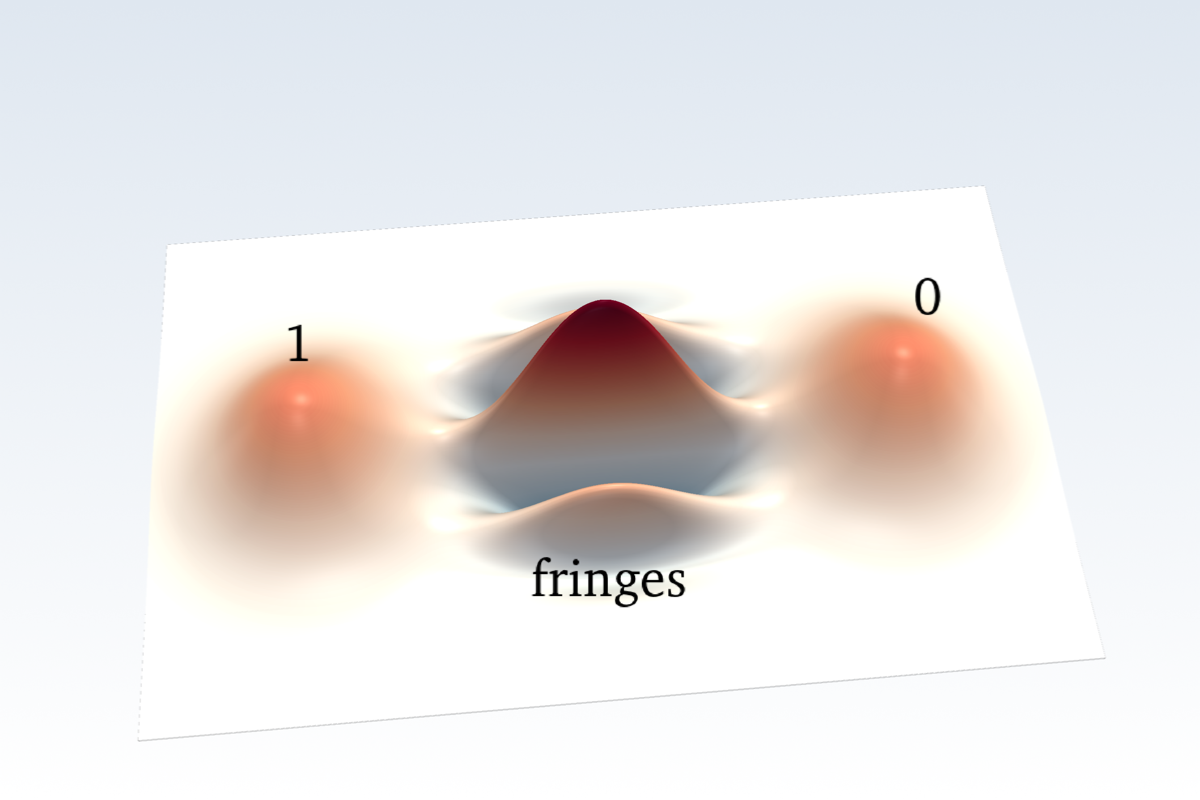
\includegraphics[height=0.42\textheight]{p07}}

\begin{document}

\begin{frame}
  \titlepage
\end{frame}

\figframe[0.62]{The device}{
  \item Memory resonator stores the qubit, $\kappa_a/2\pi = 9.3$ kHz
  \item Buffer resonator leaks on purpose, $\kappa_b/2\pi = 2.6$ MHz
  \item Coupler trades two memory photons for one buffer photon, $g_2/2\pi = 0.763$ MHz
}{p01}

\begin{frame}{The model}
  \begin{columns}[c]
    \column{0.48\textwidth}
    \[ H = g_2\big(a^2 b^\dagger + a^{\dagger 2} b\big) - \epsilon_d\big(b + b^\dagger\big) \]
    \[ L_b = \sqrt{\kappa_b}\,b, \qquad L_a = \sqrt{\kappa_a}\,a \]
    \begin{itemize}\gap
      \item Pairs out and pairs in balance at $\alpha^2 = \epsilon_d/g_2$
      \item $\alpha = 2.1$, so 4.41 photons
      \item Logical 0 and 1 are the valleys at $\pm\alpha$
    \end{itemize}
    \column{0.50\textwidth}
    \centering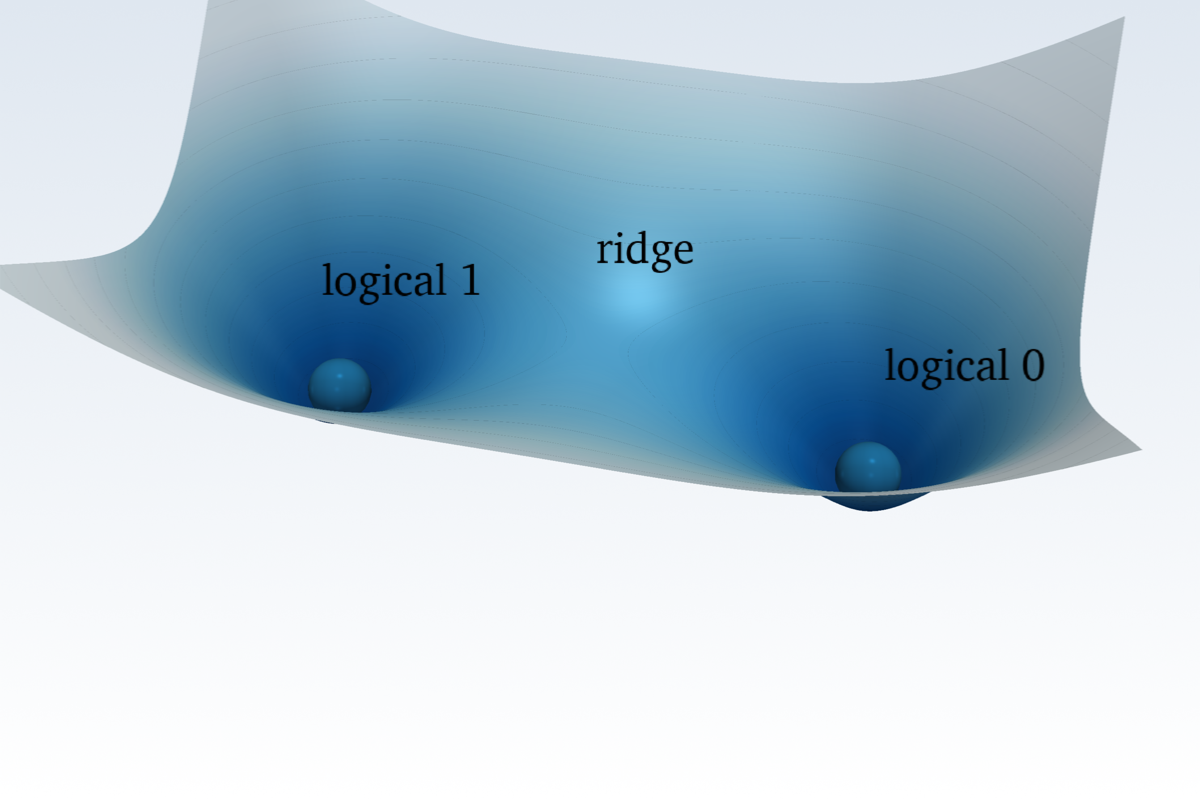
\includegraphics[width=\linewidth]{p05}
  \end{columns}
\end{frame}

\figframe{Task 1.0: Warm-up}{
  \item One-photon loss matches $4e^{-\kappa t}$ to $6\times10^{-12}$
  \item Pair loss stalls at 0.4998, the odd-parity weight
  \item Stabilization settles at $\alpha^2$ in a time $\propto 1/\kappa_2$
}{task1_0c_photon_number}

\figframe{Task 1.1: The full two-mode model}{
  \item Memory overshoots to 6.91 photons at 0.235 $\mu$s
  \item Memory and buffer ring with period 0.32 $\mu$s, linear theory 0.319 $\mu$s
  \item Memory-only model needs $\kappa_b \gg \epsilon_d$, here $\epsilon_d/\kappa_b = 1.29$
}{task1_1_vs_memory_only}

\begin{frame}{Task 1.1: Inflating a cat}
  \centering
  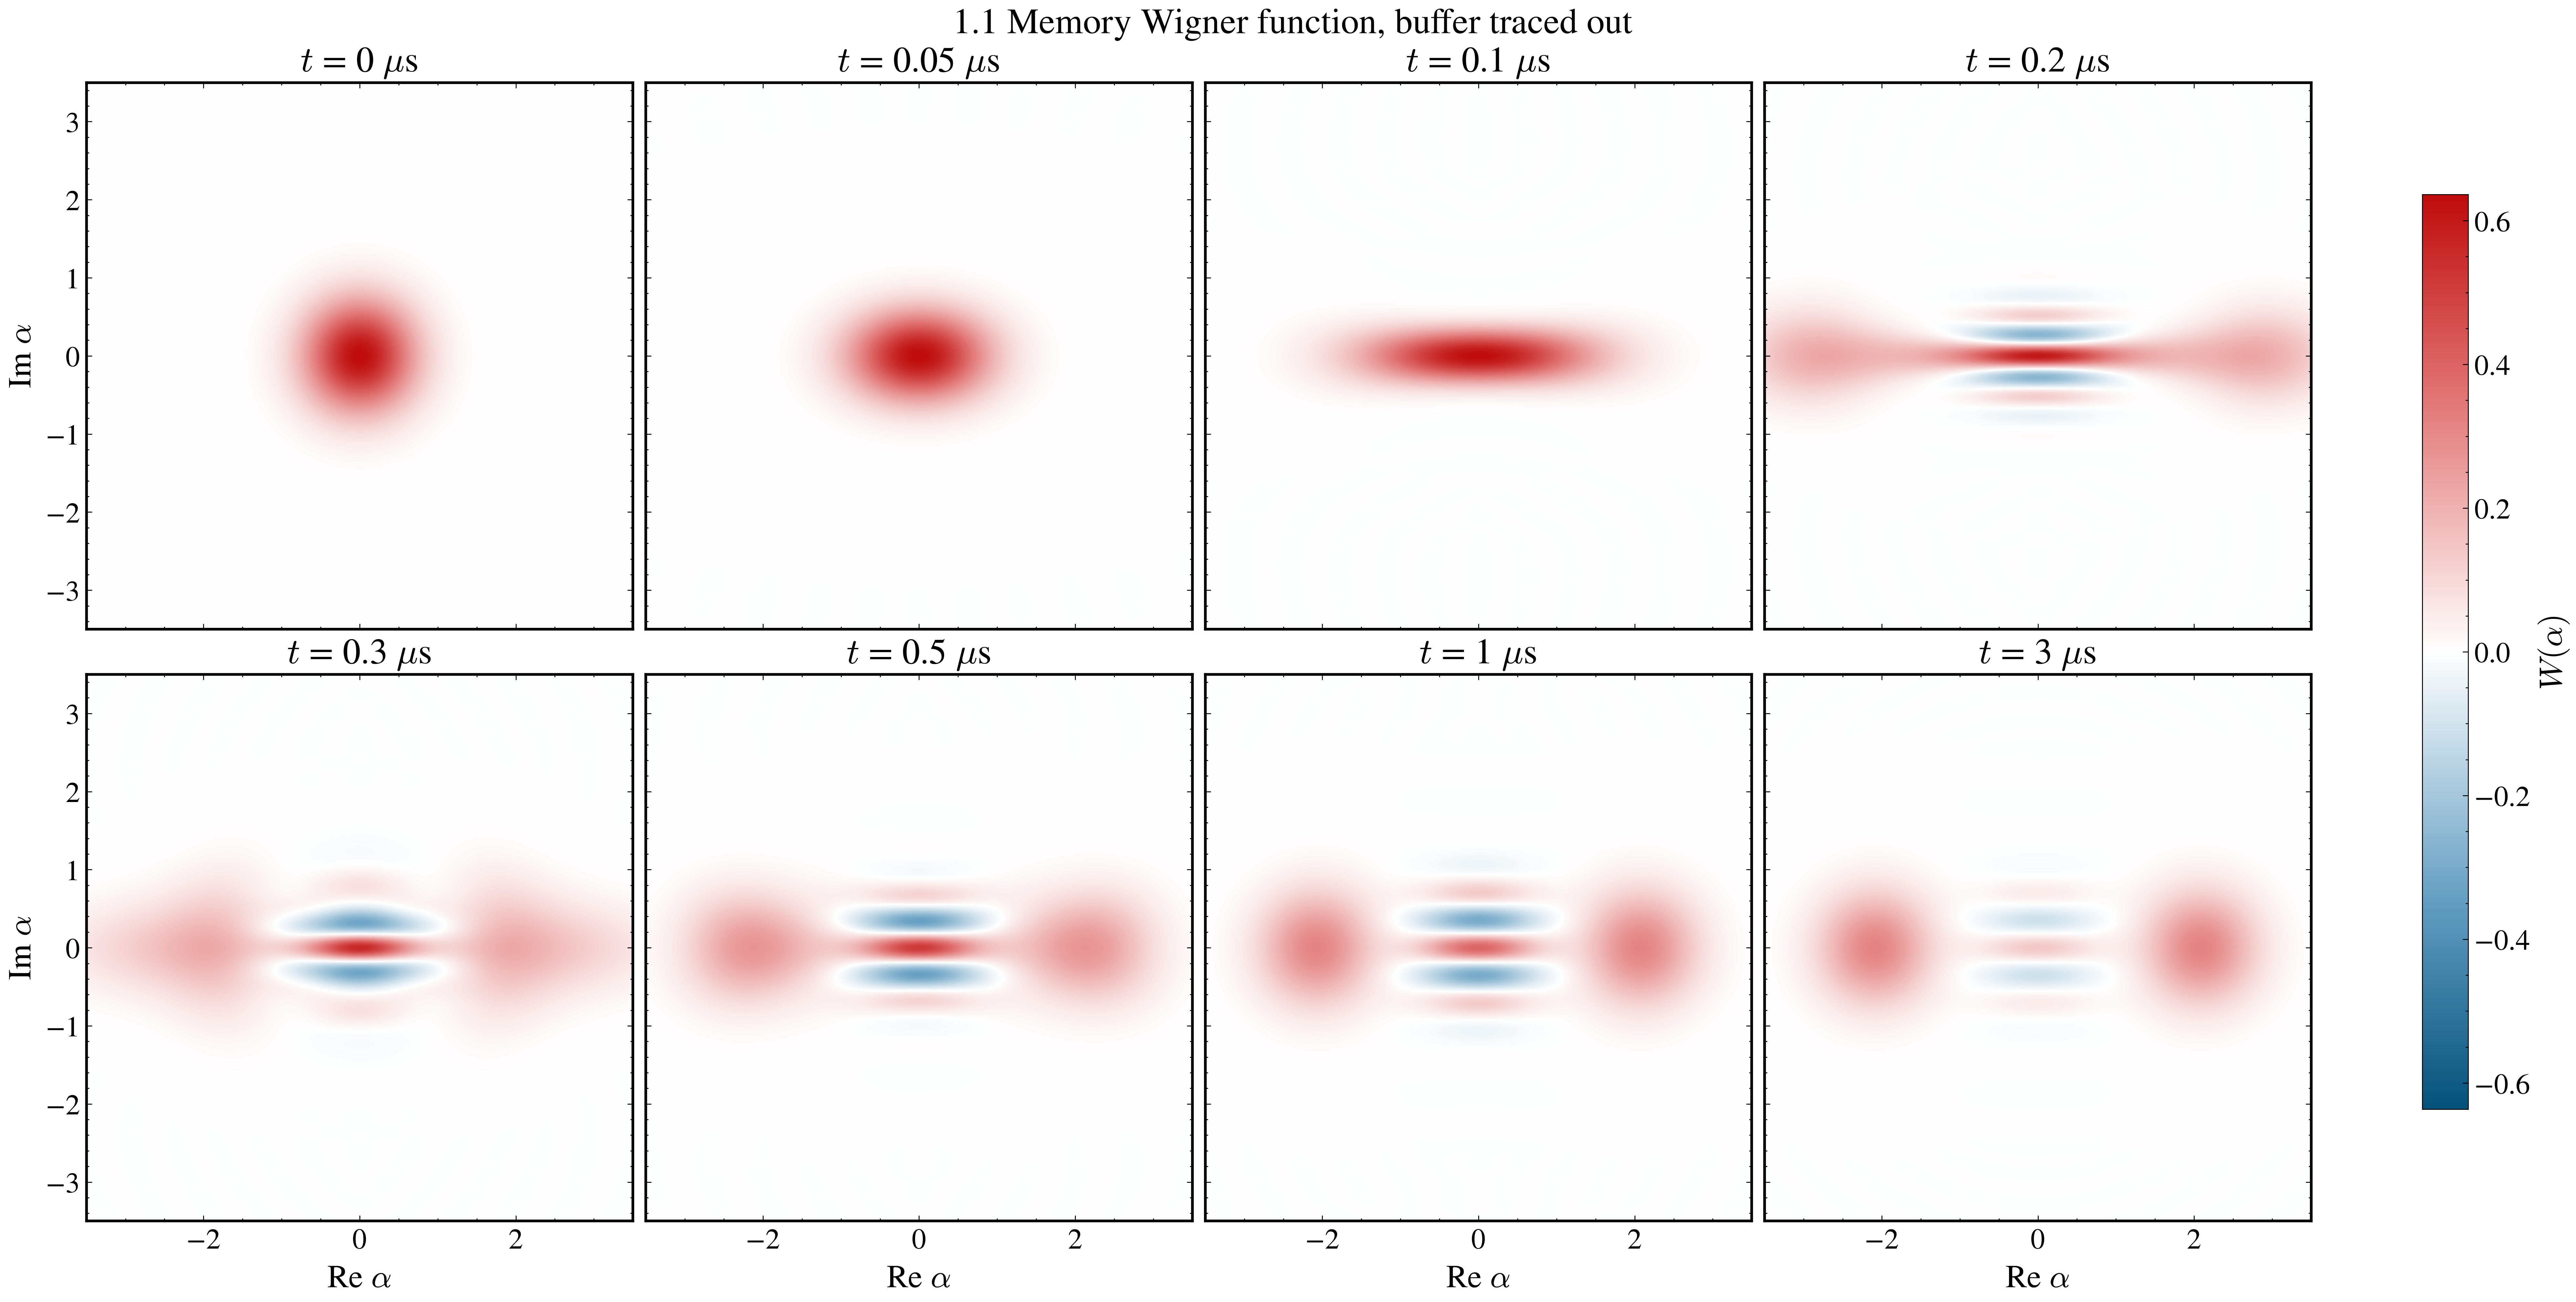
\includegraphics[width=0.94\textwidth]{task1_1_wigner}
\end{frame}

\begin{frame}{Task 1.2: Convergence study}
  \centering
  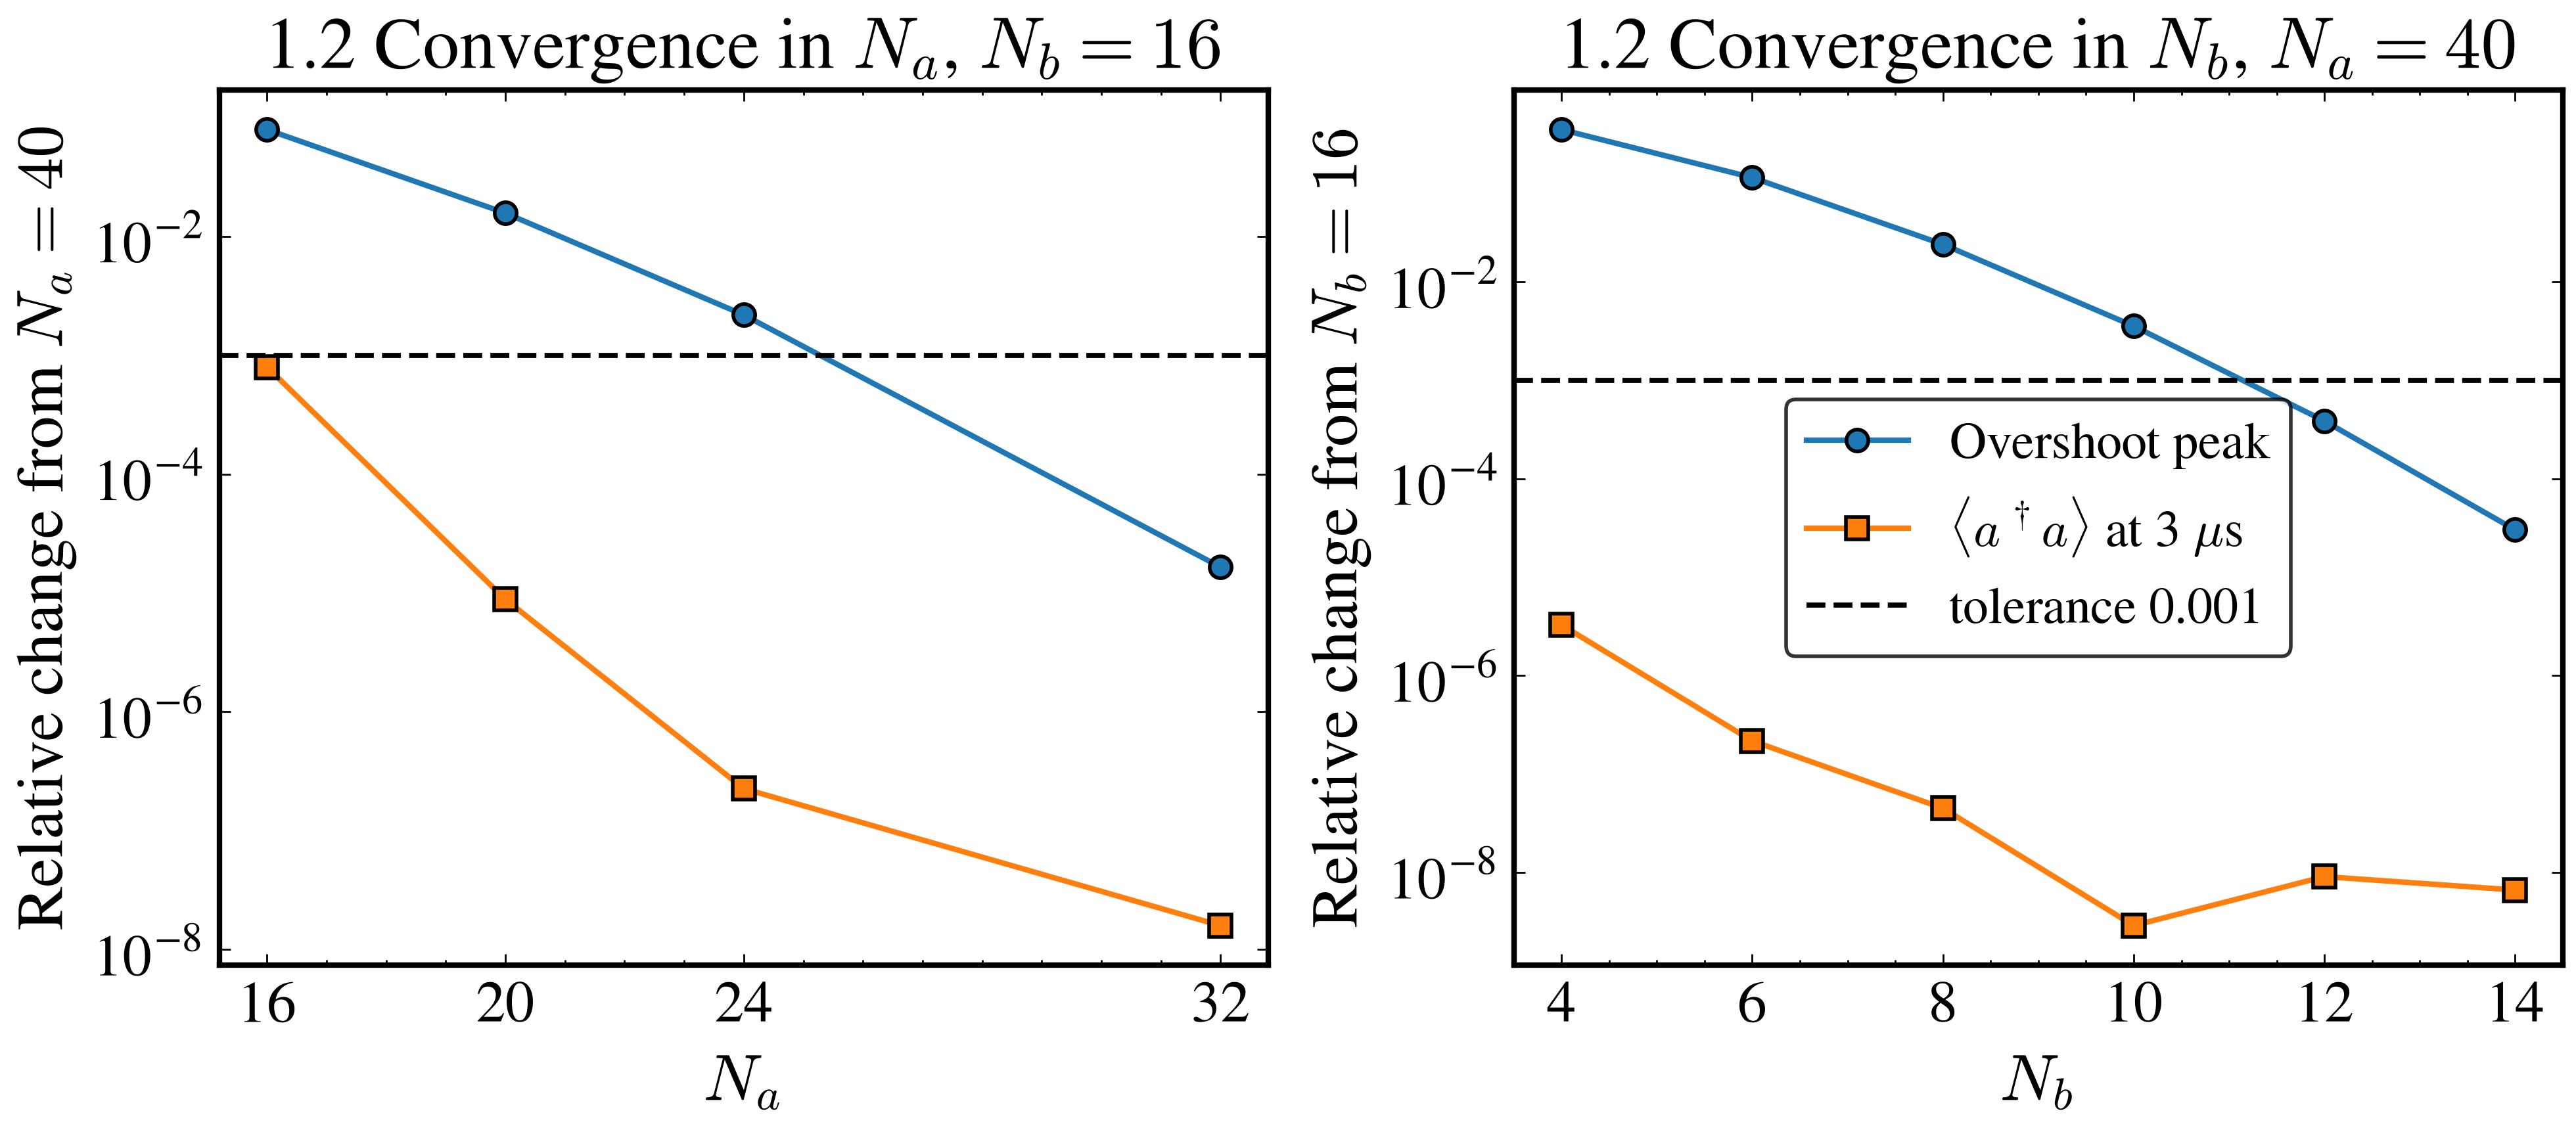
\includegraphics[width=0.86\textwidth]{task1_2_convergence}
  \begin{itemize}\gap
    \item Steady state 4.4026, 0.17\% below $\alpha^2$, converged from $16\times4$ levels
    \item Overshoot needs $32\times12$; the suggested $N_b = 6$ is 11.5\% low
  \end{itemize}
\end{frame}

\figframe{Task 1.3(a): The even cat}{
  \item Pair processes conserve parity, and the vacuum is even
  \item Fringes give $W(0) = (2/\pi)\langle P\rangle$ at every snapshot
  \item Parity lifetime 1.943 $\mu$s; superposition until 1.45 $\mu$s
}{task1_3a_cat_quantities}

\figframe{Task 1.3(b, c): Preparing $\ket{+\alpha}$}{
  \item 12 MHz, 50 ns memory pulse during inflation: $F = 0.99962$
  \item Displacing to $\beta = \alpha$ before the pump: $F = 0.999991$
  \item Cost: drive phase locked to the pump; 30$^\circ$ error gives $1 - F = 3.5\times10^{-3}$
}{task1_3b_wrong_well}

\figframe{Task 2.1: Bit-flip rate}{
  \item $\Gamma_X \propto e^{-\gamma\alpha^2}$, $\gamma = 3.02 \pm 0.04$ for $\alpha = 0.8$ to 1.4
  \item Time fits and Liouvillian eigenvalues agree to $10^{-11}$
  \item At $\alpha = 2.1$: $T_X = 2.6$ s
}{task2_1_gamma_x}

\figframe{Task 2.1: Why $\gamma$ is not 2}{
  \item Golden rule gives $\gamma = 4$; first-order loss gives 3.22
  \item A second-order path through the buffer lowers it to 3.02
  \item That path dominates past $\alpha \approx 1.6$; local $\gamma = 1.9$ at $\alpha = 2.1$
  \item Thermal photons, $n_{\rm th} = 0.1$, give $\gamma = 2.02$
}{task2_1_local_exponent}

\begin{frame}{Task 2.2: Phase-flip rate}
  \centering
  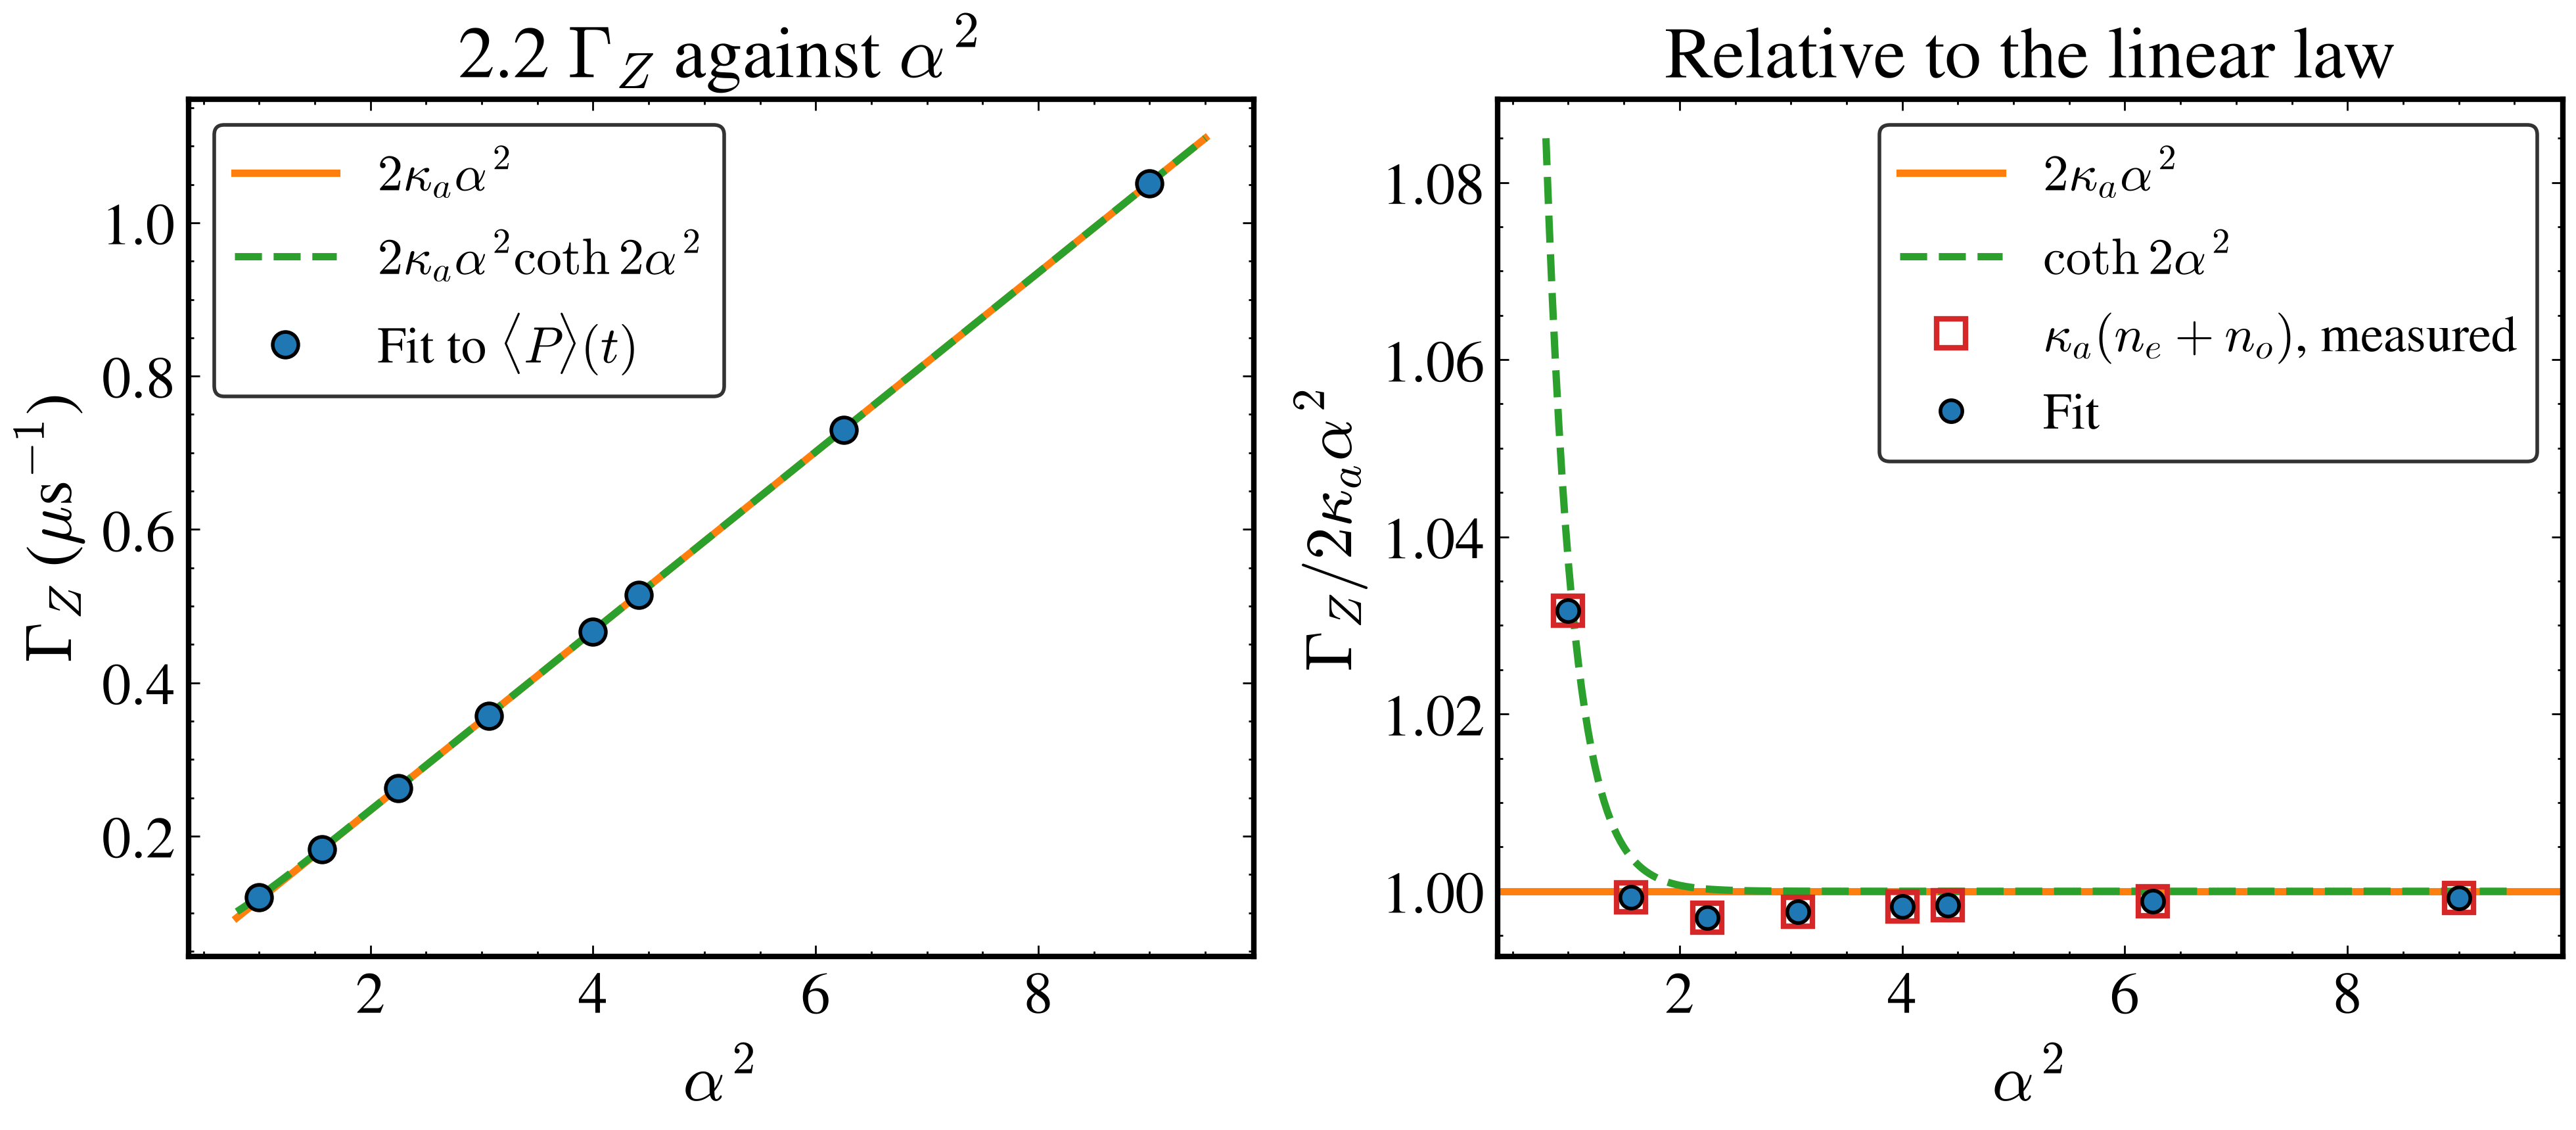
\includegraphics[width=0.80\textwidth]{task2_2_gamma}
  \begin{itemize}\gap
    \item $\Gamma_Z = 0.5146\ \mu\mathrm{s}^{-1}$ at $\alpha = 2.1$, so $T_Z = 1.94\ \mu$s; slope over $\alpha \ge 1.5$ is $0.99998 \times 2\kappa_a$
    \item Bias at $\alpha = 2.1$: $T_X/T_Z = 1.3\times10^{6}$
  \end{itemize}
\end{frame}

\figframe{Task 2.3: Readout through the buffer}{
  \item Drive $\epsilon_Z(a + a^\dagger)$ gives $\langle b\rangle = \mp\epsilon_Z/2\alpha g_2$ to 0.1\%
  \item Rings with period 0.31 $\mu$s, settled to 1\% after 0.97 $\mu$s
  \item At $\epsilon_Z = 0.1\,g_2$: 1\% error needs 146 $\mu$s of homodyne
  \item A readout with 1\% error flips the qubit with probability $1.7$ to $1.8\times10^{-3}$
}{task2_3_b_trace}

\figframe{Task 2.4: The readout trade-off}{
  \item Total error = misreading + flips caused by the readout drive
  \item Best at $\alpha = 2.1$: $3.9\times10^{-3}$, 85\% of it from flips
  \item A stronger drive only trades listening time for flips; above $0.2\,g_2$ it gets worse
}{task2_4_fom}

\figframe{Task 2.4: Raise $\alpha$ for the readout}{
  \item Drive-induced flips fall about as $e^{-2\alpha^2}$, the signal only as $1/\alpha$
  \item Reading at $\alpha = 2.5$: error $2.3\times10^{-4}$, 18 times lower
  \item Two-step turn-on cuts settling from 0.97 to 0.25 $\mu$s
  \item Circuit level: only the pair term is resonant; the rest are calibratable shifts
}{task2_4_alpha}

\begin{frame}{Summary}
  \centering
  \begin{tabular}{ll}
    \toprule
    Task & Result \\
    \midrule
    1.1 Inflation & overshoot to 6.91 photons, ringing period 0.32 $\mu$s \\
    1.2 Convergence & steady state from $16\times4$, overshoot from $32\times12$ \\
    1.3 Logical state & even cat; $\ket{+\alpha}$ with $F = 0.99962$ (pulse) or 0.999991 \\
    2.1 Bit flips & $\gamma = 3.02$ for $\alpha \le 1.4$; $T_X = 2.6$ s at $\alpha = 2.1$ \\
    2.2 Phase flips & $T_Z = 1.94\ \mu$s at $\alpha = 2.1$, slope $0.99998\times2\kappa_a$ \\
    2.3 Readout & contrast within 0.1\% of theory, settles in 0.97 $\mu$s \\
    2.4 Readout optimization & read at $\alpha = 2.5$: error 18 times lower; settles in 0.25 $\mu$s \\
    \bottomrule
  \end{tabular}

  \vspace{1.2em}
  \small Code, plots and write-up: github.com/yubrajbhandari923/DuQuantum, branch ak-changes
\end{frame}

\end{document}
